\chapter{Propagation of a wave over a conical island (conical\_island)}

\section{Purpose}

To compare \telemac{2D} simulation with an experiment by Costas E
Synolaki~\cite{Costas2007}.

\section{Description}

\subsection{Geometry and mesh}

Size of the model: rectangle (25~m $\times$ 30~m)

Water depth: $h$ = 0.32~m

Figure~\ref{fig:island:geometry} shows the geometry of the study.

\begin{figure}[H]
\centering
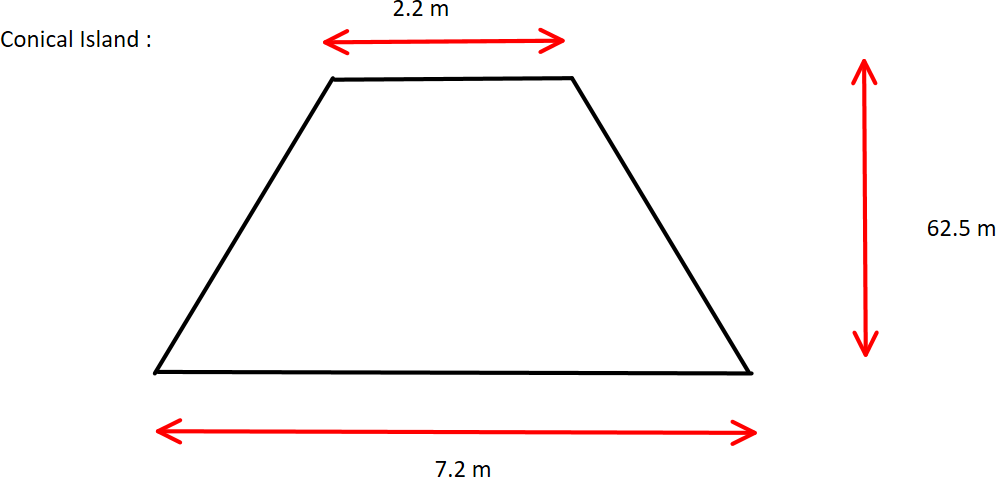
\includegraphics[width=.6\textwidth]{img/geometry.png}
\caption{Geometry of the study.}\label{fig:island:geometry}
\end{figure}

\begin{itemize}
%\item Nodes: 4,996
%\item Elements: 9,742
\item Nodes: 4,995
\item Elements: 9,741
\end{itemize}

Figure~\ref{fig:island:mesh} displays the mesh.

\begin{figure}[H]
\centering
\includegraphicsmaybe{[width=.6\textwidth]}{../img/Mesh.png}
\caption{Mesh of the study.}\label{fig:island:mesh}
\end{figure}

Figure~\ref{fig:island:bathy} displays the bathymetry.

\begin{figure}[H]
\centering
\includegraphicsmaybe{[width=.6\textwidth]}{../img/Bathy.png}
\caption{Bathymetry of the study.}\label{fig:island:bathy}
\end{figure}


\subsection{Boundaries}

Figure~\ref{fig:island:boundaries} shows what types of boundaries are used for
this study.
\begin{figure}[H]
\centering
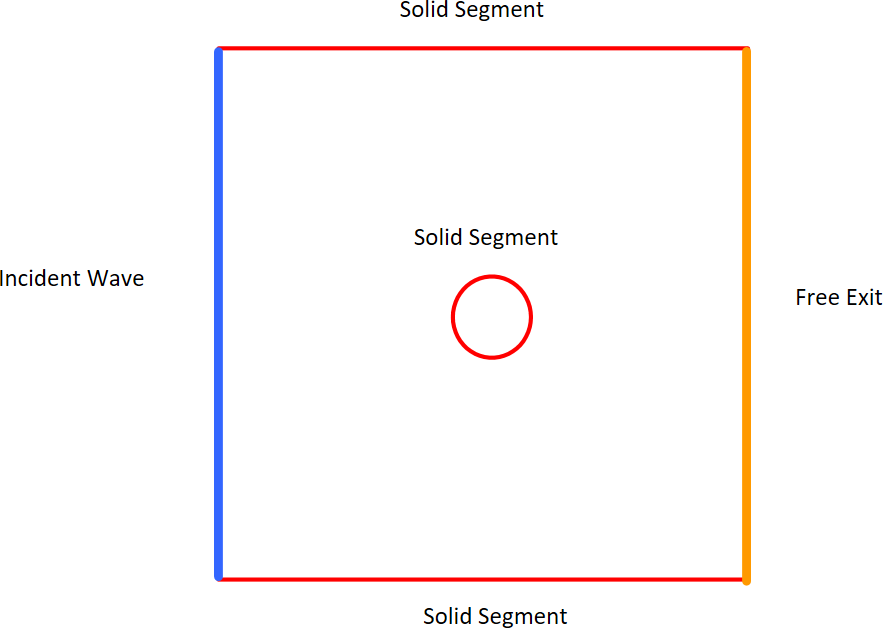
\includegraphics[width=.6\textwidth]{img/boundaries.png}
\caption{Boundaries of the study.}\label{fig:island:boundaries}
\end{figure}

Equation for the free surface:
$\eta(t)= h+H.sech^{2}(\sqrt(3H/(4h^{3})).ct-X_{1})$ with $H/h=0.045$

Bottom:
\begin{itemize}
\item Bottom Friction: Chézy's formula,
\item Friction Coefficient: 100~m$^{1/2}$/s.
\end{itemize}

\subsection{Physical Parameters}

Turbulence: Constant viscosity equal to zero.

\subsection{Numerical parameters}

\begin{itemize}
\item Type of element: P1 triangle for $h$ and for velocity
%\item Type of advection: Implicit N scheme on non conservative equation + SUPG decentring on velocities PSI distributive scheme, mass-conservative + modified SUPG on depth
%\item Solver: GMRES
%\item Accuracy: $10^{-6}$
\item Finite volume scheme: Kinetic order 2
\item Desired Courant number: 0.8
%\item Implicitation for depth: 1
%\item Implicitation for velocity: 0.6
\item Option for liquid boundaries: Thompson
\end{itemize}

Time Date:
\begin{itemize}
%\item Time step 0.005~s,
%\item Simulation duration 40~s.
\item Time step 0.05~s,
\item Simulation duration 20~s.
\end{itemize}

\section{Results}

We compare the model and the analytical solution free surface at gauges 6, 9, 16 and 22.

Figure~\ref{fig:island:exp} displays the experiment we are comparing to.
\begin{figure}[H]
\centering
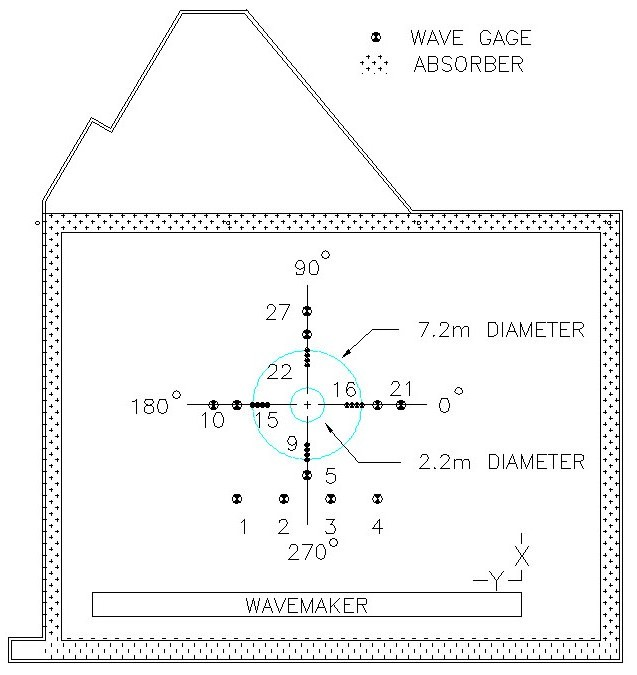
\includegraphics[width=.6\textwidth]{img/experiment.jpg}
  \caption{Boundaries of the study.}\label{fig:island:exp}
\end{figure}

Figure~\ref{fig:island:res} shows comparison between experimental values and
the simulation at specific points.
\begin{figure}[H]
  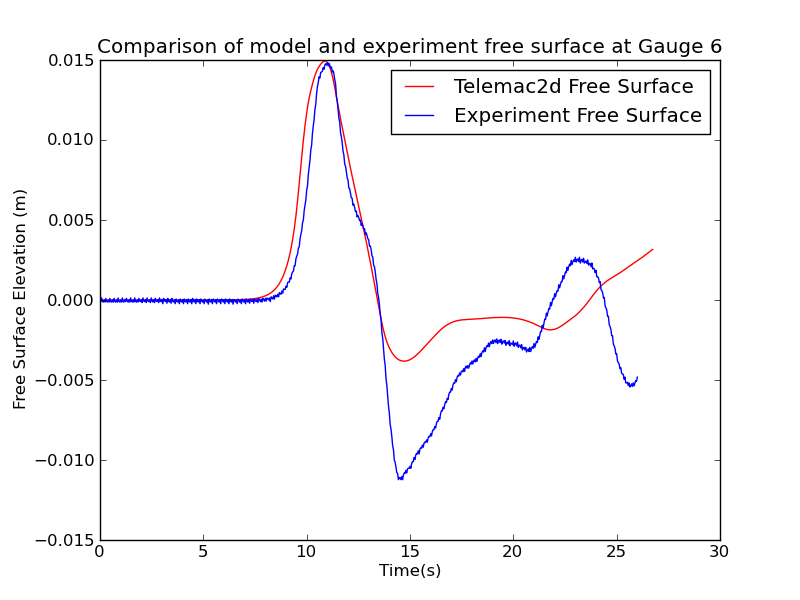
\includegraphics[width=.6\textwidth]{img/gauge6.png}
  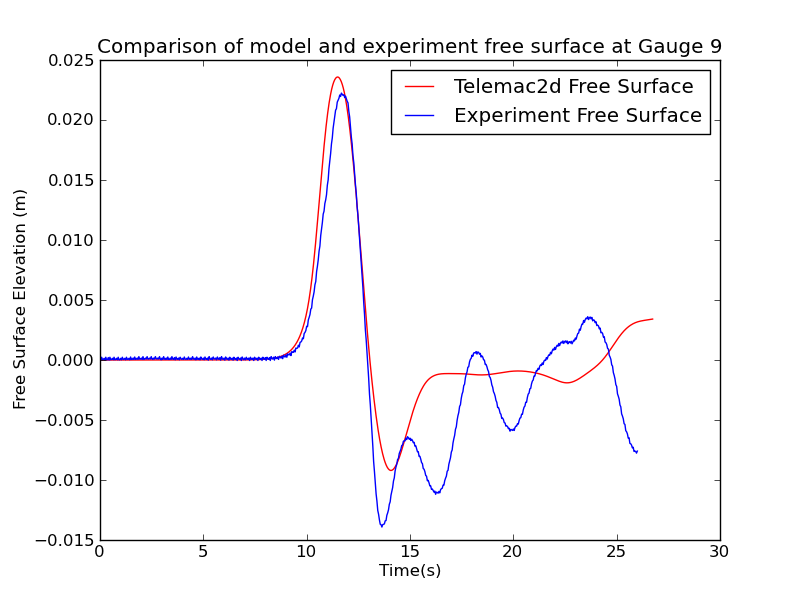
\includegraphics[width=.6\textwidth]{img/gauge9.png}
  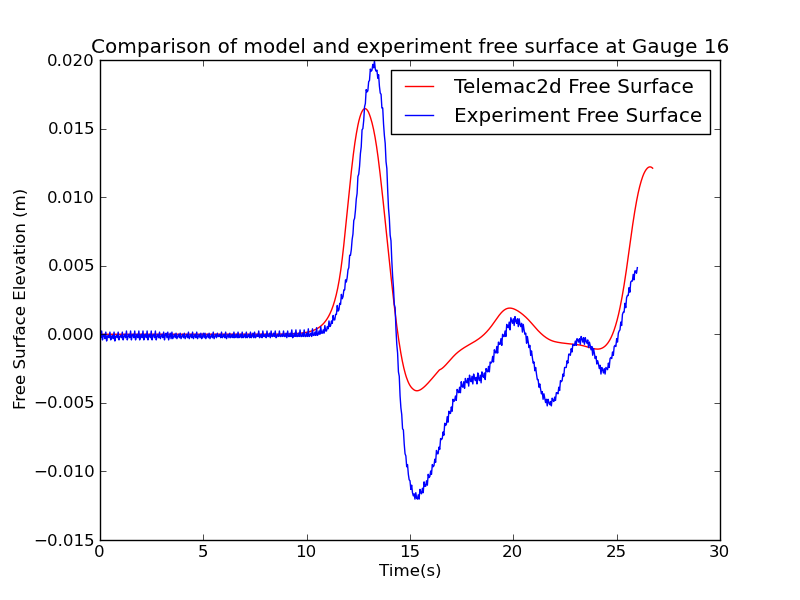
\includegraphics[width=.6\textwidth]{img/gauge16.png}
  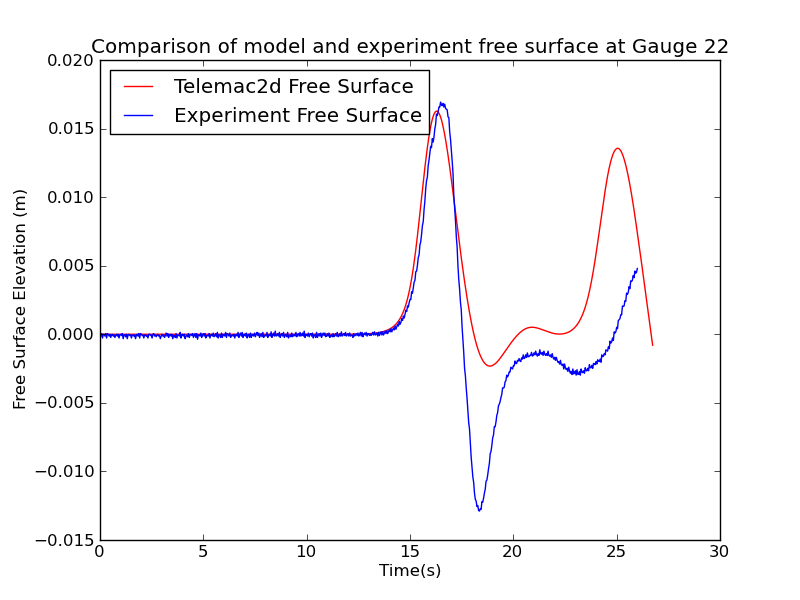
\includegraphics[width=.6\textwidth]{img/gauge22.png}
  \caption{Comparaison with experimental data at the some gauges.}\label{fig:island:res}
\end{figure}
